%!TEX root = ../article.tex
\subsection{Individual View}
After observing an overview on data similarities, users may need to drill down to a few individuals of interest for detailed examination.
We develop the Individual View for users to explore and compare the different individuals over time (\textbf{T6}).
Specifically, our goal is to identify the important features at different time steps and their relationship to raw feature values (\textbf{T2}, \textbf{T4}).


\begin{figure}[t]
	\centering
    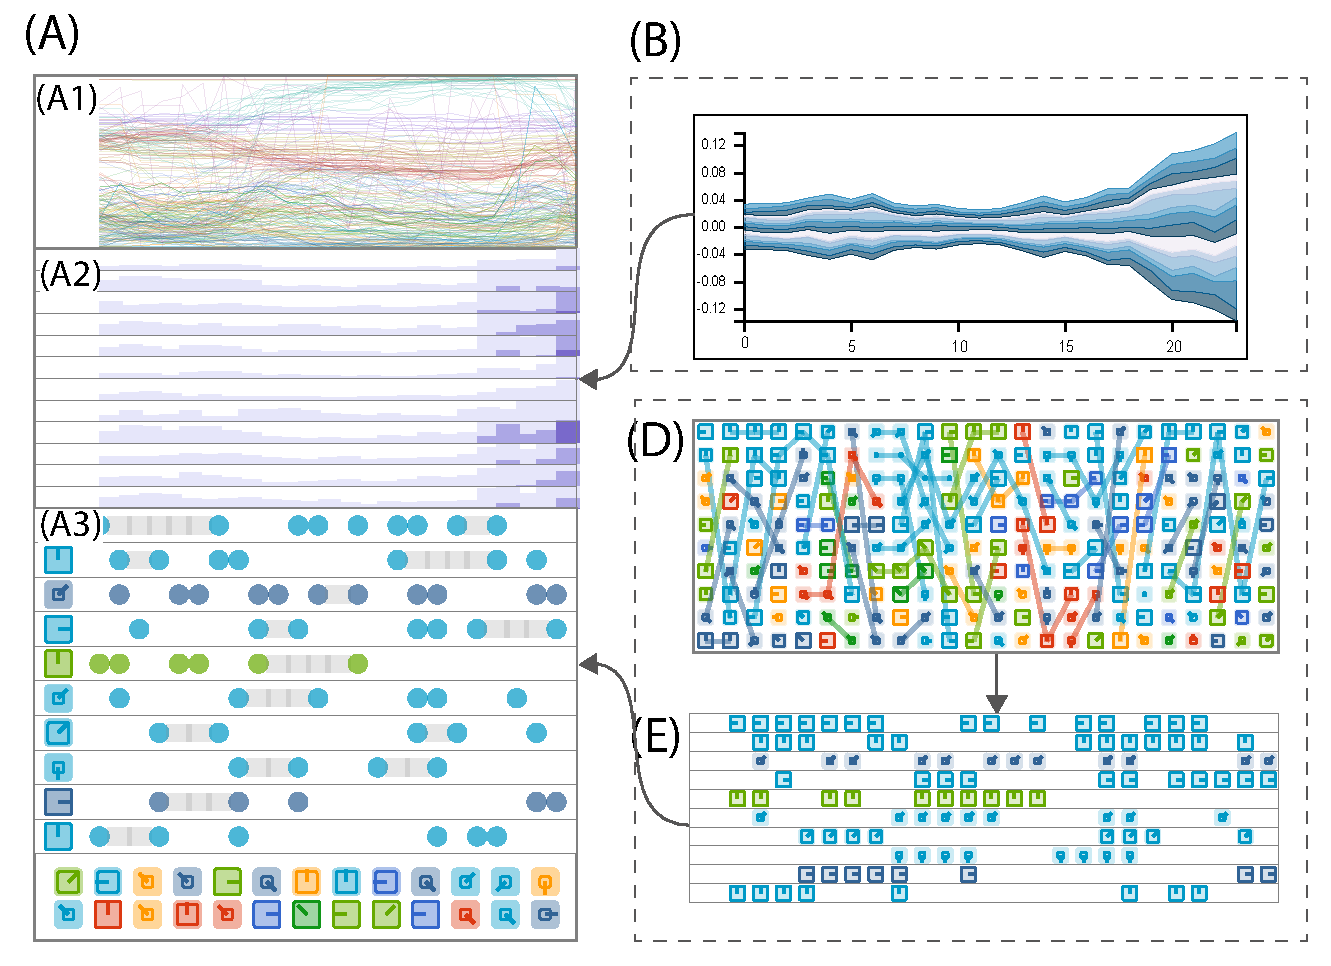
\includegraphics[width=0.49\textwidth]{pictures/design/alternative_design.pdf}
	\vspace{-3mm}
	\caption{Individual design and the alternative designs. A) Individual View. A1) Feature Trend Chart; A2) Cluster Importance Chart; A3) Top Features Chart. B) themeriver as the alternative design of the Cluster Importance Chart; C) and D) node-like sequence and node sequence as the alternative design of Top Features List.}
	\label{fig:individual_view}
	\vspace{-4mm}
\end{figure}


The selected individual cases are visualized as several stacks of cells as in Fig.~\ref{fig:individual_view}A to show the detailed information.
Each cell consists of three components: the Feature Trend Chart, the Cluster Importance Chart, and the Top Feature List from top to bottom as shown in Fig.~\ref{fig:individual_view}A$_1$,A$_2$,A$_3$.
The top component is the Feature Trend Chart, which is a multi-line chart that depicts how different features' values change over time. 
The x-axis represents the time where time steps increase from left to right, and the y-axis represents normalized feature values where the feature value increases from bottom to top ranging between 0 and 1.
Each line represents a feature and the line color encodes feature category the same as in the Cluster View.
The corresponding lines will be highlighted when hovering on any feature groups in the Cluster View to enable users to focus on the features in the current context and avoid visual clutter.

The middle component is the Cluster Importance Chart, which is a list of stacked bar charts that summarize how each feature group's gradient changes over time.
Each feature group is represented as a stacked bar chart and aligned vertically in the same order as the Cluster View.
For each bar chart, the x-axis represents time the same as in the Feature Trend Chart, and each bar represents the averaged gradient for the corresponding feature group at one time step. 
We use both the bar height and bar color to encode the gradient value.
As shown in  Fig.\ref{fig:individual_view}A$_3$, the first visual channel to encode gradient value is bar height where a greater height indicates a larger gradient value.
When the gradient value exceeds a certain limit, we clip the bar and overlay another darker bar with the same height as the clipped part at the same position for better vertical space efficiency.
We have also considered other design choices such as a themeriver (Fig.\ref{fig:individual_view}B) in which each colored flow indicates a feature group. 
However, users may feel it is difficult to compare different feature groups, and it requires more space when the gradient is large.
Thus, we abandon this alternative choice and adopt the current design.

Though the Cluster Importance Chart provides an overview of how each feature cluster's importance changes over time, users still need to link this component to the Cluster View to observe which features are considered important by the model.
We first design a Top Feature List as shown in Fig.~\ref{fig:individual_view}D. We rank the features by importance at each timestamp, and only visualize the top N features by layout feature glyph for each timestamp in order to alleviate the burden on users. If a feature is ranked in the top N important features for more than two consecutive timestamps, we use a link to connect the adjacent glyph. However, this design also leads to serious visual clutter caused by the link overlap, since the rank of features are frequently only slightly changed by timestamps. 
To alleviate the user's mental burden, we improve the Top Feature List as Fig.~\ref{fig:individual_view}A$_3$ shows.
In this component, we visualize the top $N$ features that have the largest average gradients over time. Each feature is represented as a horizontal row and the glyph appears at the timestamps when this feature is ranked in the top $K$($K>N$) most important features (Fig.\ref{fig:individual_view}E). To further simplify the visual design, the feature glyph is positioned at the beginning to indicate feature category. 
As a feature has different gradients over time, the importance ranking of a feature can also vary at different steps.
For each row, we use two colored circles linked with gray lines to indicate at which time steps the corresponding feature is ranked in the top $K$($K>N$) mostly important features.
The circle color is consistent with the feature glyph color.
To make the Top Feature List space efficient, we only show ten feature rows by default, and other features are collapsed as feature glyph rows as shown in the bottom at Fig.\ref{fig:individual_view}A$_3$.
Users can click the glyph rows to select different features to analyze.


The three components enable users to observe which features are considered important by the model over time and how the importance is related to feature value changes.
Users can also append multiple cells to the Sequence View to compare different sequences side by side. 
When the number of cells becomes large, we use dbscan to cluster the similar individual cases into one stacked cells with one randomly selected case presented at the top of stack.